%compile with pdflatex on papeeria

\documentclass[a4paper,12pt]{article}


\usepackage{fontawesome}

\usepackage{fancyhdr}
\usepackage{fancyheadings}
\usepackage[ngerman,german]{babel}
\usepackage{german}
\usepackage[utf8]{inputenc}
%\usepackage[latin1]{inputenc}
\usepackage[active]{srcltx}
%\usepackage{algorithm}
%\usepackage[noend]{algorithmic}
\usepackage{amsmath}
\usepackage{amssymb}
\usepackage{amsthm}
\usepackage{bbm}
\usepackage{enumerate}
\usepackage{graphicx}
\usepackage{ifthen}
\usepackage{listings}
\usepackage{enumitem}
%\usepackage{struktex}
\usepackage{hyperref}
\usepackage{tikz}
\usepackage{float}
\usepackage{subcaption}
\usepackage{array}
\captionsetup{compatibility=false}
\captionsetup[subfigure]{labelformat=empty}

\usepackage{pgfplots}
\pgfplotsset{compat=1.15}
\usepackage{mathrsfs}
\usetikzlibrary{arrows}

\definecolor{ccqqqq}{rgb}{0.8,0,0}
\definecolor{kolorwykresu}{rgb}{0.07,0.04,0.56}

\pagenumbering{gobble}

\usepackage{tabularray}
\usepackage{multirow}
\usepackage{booktabs,tabularx}

\DeclareMathSymbol{\shortminus}{\mathbin}{AMSa}{"39}

\renewcommand\tabularxcolumn[1]{m{#1}}% for vertical centering text in X column

\newcolumntype{L}[1]{>{\raggedright\let\newline\\\arraybackslash\hspace{0pt}}m{#1}}
\newcolumntype{C}[1]{>{\centering\let\newline\\\arraybackslash\hspace{0pt}}m{#1}}
\newcolumntype{R}[1]{>{\raggedleft\let\newline\\\arraybackslash\hspace{0pt}}m{#1}}

\newcolumntype{Y}{>{\centering\arraybackslash}X}



\newcounter{aufgabencounter}
\newcommand{\aufgabeNr}{\stepcounter{aufgabencounter}{\theaufgabencounter}}


%%%%%%%%%%%%%%%
%% Aufgaben-COMMAND
\newcommand{\Aufgabe}[1]{
  {
  \vspace*{0.5cm}
  \textsf{\textbf{Aufgabe \aufgabeNr} #1}
  \vspace*{0.2cm}
  
  }
}

%%%%%%%%%%%%%%%%%%%%%%%%%%%%%%%%%%%%%%%%%%%%%%%%%%%%%%
%%%%%%%%%%%%%% EDIT THIS PART %%%%%%%%%%%%%%%%%%%%%%%%
%%%%%%%%%%%%%%%%%%%%%%%%%%%%%%%%%%%%%%%%%%%%%%%%%%%%%%
\newcommand{\Fach}{2. Klausur aus der Mathematik}
\newcommand{\Name}{}
\newcommand{\datum}{}
\newcommand{\Matrikelnummer}{}
\newcommand{\Semester}{Q12/2}
\newcommand{\Uebungsblatt}{} %  <-- UPDATE ME
%%%%%%%%%%%%%%%%%%%%%%%%%%%%%%%%%%%%%%%%%%%%%%%%%%%%%%
%%%%%%%%%%%%%%%%%%%%%%%%%%%%%%%%%%%%%%%%%%%%%%%%%%%%%%

\setlength{\parindent}{0em}
\topmargin -1.0cm
\oddsidemargin 0cm
\evensidemargin 0cm
\setlength{\textheight}{9.2in}
\setlength{\textwidth}{6.0in}

%%%%%%%%%%%%%%%
%% Aufgaben-COMMAND
%\newcommand{\Aufgabe}[1]{
%  {
%  \vspace*{0.5cm}
%  \textsf{\textbf{Aufgabe #1}}
%  \vspace*{0.2cm}
%  
%  }
%}
%%%%%%%%%%%%%%
\hypersetup{
    pdftitle={\Fach{}: Übungsblatt \Uebungsblatt{}},
    pdfauthor={\Name},
    pdfborder={0 0 0}
}

\lstset{ %
language=java,
basicstyle=\footnotesize\tt,
showtabs=false,
tabsize=2,
captionpos=b,
breaklines=true,
extendedchars=true,
showstringspaces=false,
flexiblecolumns=true,
}

\title{Übungsblatt \Uebungsblatt{}}
\author{\Name{}}

\begin{document}

\fancyhead{}
\fancyhead[C]{
\includegraphics[height=2.5cm]{lukasLogo.png}
\vspace{2cm}
}

\thispagestyle{fancy}

\lhead{
%\vspace{1cm}
  \sf \LARGE \Fach{} %\small \Name{} - \Matrikelnummer{}
}
\rhead{\sf \Semester{}   \datum{}}

\vspace*{0.2cm}

\vspace{4cm}
Alle Lösungen müssen mit Nebenrechnungen und Begründungen nachvollziehbar sein!

%\rhead{\sf \Semester{} }
\vspace*{0.2cm}

%\begin{center}
%%\LARGE \sf \textbf{Übungsblatt \Uebungsblatt{}}
%\end{center}
%\vspace*{0.2cm}

%%%%%%%%%%%%%%%%%%%%%%%%%%%%%%%%%%%%%%%%%%%%%%%%%%%%%%
%% Insert your solutions here %%%%%%%%%%%%%%%%%%%%%%%%
%%%%%%%%%%%%%%%%%%%%%%%%%%%%%%%%%%%%%%%%%%%%%%%%%%%%%%

\vspace{1cm}
  Name: \underline{\hspace{7cm}}
  \hfill
  Datum: \underline{\hspace{4cm}}

\vspace{0.8cm}

Zeit: 90 Minuten
%\vspace{0,5cm}Die Rechenwege müssen nachvollziehbar sein!
%
%\vspace{0,5cm} {TEIL A} - ohne Hilfsmittel - Bearbeitungszeit 30 Minuten
\vspace {0.8cm}
% 
%GEOMETRIE


\begin{center}
  \begin{tblr}{
      width=1\linewidth,
      colspec = {Q[c,6em]Q[c,4em]Q[c,4em]Q[c,4em]Q[c,4em]Q[c,6em]},
      rowspec = {Q[m]Q[m]Q[m]Q[m]Q[m]Q[m]},
      colsep = 0mm,
      %row{1} = {2em,azure2,fg=white,font=\large\bfseries\sffamily},
      row{1} = {2em,font=\large\bfseries\sffamily},
      hlines, vlines,
    }
    \textbf{Aufgabe} & \textbf{1} & \textbf{2} & \textbf{3} & 
    \textbf{4} & \textbf{Gesamt} \\
    {Mögliche \\ Punkte} & {7} & {18} & {10} & 12 & 47 \\
    {Erreichte \\ Punkte} &  &  &  &  &  \\
  \end{tblr}
\end{center}

\vspace{5cm}
%\centerline{\huge\bfseries\sffamily Viel Erfolg !!!}

\newpage


\vspace{1,5cm} 
\begin{center}
  {\bf TEIL A} - ohne Hilfsmittel - Zeit 30 min
\end{center}
\vspace {0,2cm}
 

\Aufgabe{(2BE+2BE+2BE)}
Untenstehende Abbildung zeigt den Graphen einer Funktion $f$.
\begin{center}
\includegraphics[width=8.789cm]{Q12_2Klausur20230301_1.jpg}
\end{center}
\begin{enumerate}[label={\alph*)}]
  \item Skizzieren Sie den Graphen der Ableitungsfunktion $f'(x)$ in der Abbildung.
  \item Skizzieren Sie den Graphen einer möglichen Stammfunktion $F(x)$ in der Abbildung.
  \item Begründen Sie, an welchen Stellen jede Stammfunktion von $f$ ein Minimum oder Maximum hat.
\end{enumerate}

\Aufgabe{}
\begin{enumerate}[label={\alph*)}]
  \item Bestimmen Sie eine ganzrationale Funktion höchstens fünften Grades, deren Graph bzgl. der $y$-Achse symmetrisch ist und in $P(-1|1)$ eine Wendetangente mit der Steigung 4 hat.
  \item Geben Sie einen Funktionsterm einer Funktion $f$ an, dessen Graph streng monoton steigt und rechtsgekrümmt ist.
\end{enumerate}

\Aufgabe{}
In München fahren geschätzt 3\% der Fahrgäste schwarz.
\begin{enumerate}[label={\alph*)}]
  \item Stellen Sie einen Term auf, mit dem berechnet werden kann, wie viele Fahrgäste ein Kontrolleur wenigstens kontrollieren muss, um mit einer Wahrscheinlichkeit von mehr als 90\% wenigstens einen Schwarzfahrer zu erwischen.
  \item Erläutern Sie, was mit folgendem Term berechnet wird $\bigl( \begin{smallmatrix}10 \\ 2 \end{smallmatrix} \bigr) \cdot 0,97^8 \cdot 0,03^2  $
\end{enumerate}


\Aufgabe{}
Gegeben ist eine Zufallsgröße $X$, die die Werte $x_i = \{-2; 0; 2; 4\}$ annimmt.\\
Dem untenstehenden Histogramm kann man die Wahrscheinlichkeitswerte $P(X = x_i)$ entnehmen


\begin{figure}[H]
  \centering
\begin{tikzpicture}[>=latex, line cap=round, line join=round,>=triangle 45]
\begin{axis}[
  %unit vector ratio=1 10,
  axis x line=center,
  axis y line=center,
  axis line style = thick,
  xtick align=inside,
  %extra x tick style={tick style={very thick}}
  xtick={-4,-2,0,2,4},
  ytick={0,0.1,0.2,0.3,0.4},
  xtick style=thick,
  ytick style=thick,
  xticklabels={,,},
  extra x ticks={-2,0,2,4},
  bar width=1cm,
  %xticklabel style={anchor=south west},
  %minor x tick num=1,
  %minor y tick num=1,
  %minor tick num = 1,
  x=1cm,    %größe der kästchen in x-richtung
  y=10cm,    %größe der kästchen in y-richtung
  xlabel={$x$},
  ylabel={$P(X=x)$},
  ymajorgrids=true,
  xlabel style={below right},
  ylabel style={below right},
  %xmajorgrids=true,
  xmin=-4,
  xmax=5,
  ymin=0,
  ymax=0.4]

\addplot[ybar,fill=blue,fill opacity=0.2] coordinates {
        (-2,0.2)
        (0,0.3)
        (4,0.2)
    };
\end{axis}
\end{tikzpicture}
\end{figure}

Ergänzen Sie den zu $x_i=2$ gehörenden Wahrscheinlichkeitswert im Histogramm und ermitteln Sie näherungsweise den Erwartungswert der Zufallsgröße.

\Aufgabe{}
Gegeben sind die Punkte $A (0|0|0)$ und $ C (5|3|4)$ sowie die Gerade

\[
       g: \vec{X} = \begin{pmatrix}10 \\ -3 \\-4 \end{pmatrix} 
                  + \lambda \begin{pmatrix}5 \\ -3 \\-4 \end{pmatrix}          
\] 
$(\lambda \in \mathbb{R})$

\begin{enumerate}[label={\alph*)}]
\item Zeigen Sie, dass $ g$  eine Mittelsenkrechte von $A$ und $C$ ist.
\item  Die Punkte A und C bilden zusammen mit zwei auf g liegenden Punkten das Quadrat
 $ABCD$. Bestimmen Sie die Koordinaten von B und D.
\end{enumerate}
%\begin{flushright}7 BE \end{flushright}
    \marginpar{7 BE}

\vspace {0,5cm}

\newpage
\begin{center}
  {\bf TEIL B} - Zeit 120 min
\end{center}
\vspace {0,2cm}

\setcounter{aufgabencounter}{0}

\Aufgabe{(4BE + 3BE)}
Die normale Körpertemperatur eines gesunden Menschen liegt bei 36,5°C.  Die Funktion $f$ mit $f(x) = x \cdot e^{-0,1x} + 36,5$ beschreibt modellhaft den Verlauf einer Fieberkurve bei einem Erkrankten.  Dabei ist $x$ die Zeit in Stunden nach Ausbruch der Krankheit und $f(x)$ die Körpertemperatur in Grad Celsius. Der Graph der Funktion ist in der Abbildung dargestellt.

\begin{center}
\includegraphics[width=8.789cm,height=8.65cm]{Q11_2Klausur_2chart.png}
\end{center}

\begin{enumerate}[label={\alph*)}]
  \item Berechnen Sie die maximale Körpertemperatur $T_{max}$ sowie den Zeitpunkt $x_{max}$, zu dem diese Temperatur erreicht wird.\\
(Antwortsatz!)\\
\\
    {[ Teilergebnis zur Kontrolle: $f'(x) = (1-0,1x) \cdot e^{-0,1x}$ ]}
  \item Bestimmen Sie den Zeitpunkt $x_0$, an dem die Körpertemperatur am stärksten abnimmt, und begründen Sie Ihren Rechenweg!
\end{enumerate}


\Aufgabe{(1BE + 3BE + 8BE + 6BE)}
%\textbf{Untersuchung einer Logarithmusfunktion}\\

Gegeben ist die Funktion $f$ mit $f(x)=1+\frac{3}{x}+\frac{3 \ln x}{x}$.

\begin{enumerate}[label={\alph*)}]
  \item Bestimme die Definitionsmenge.
  \item Untersuche das Verhalten von $f$ an den Grenzen des Definitionsbereiches. Gib die Gleichungen der Asymptoten an.
  \item Untersuche $G_f$ auf Monotonie- und Krümmungsverhalten. Gib die Extremstellen und Wendepunkte an.\\
    {[ Teilergebnis zur Kontrolle: $f'(x) = \frac{-3 \ln x}{x^2}$ ]}
  \item Bestimme die Gleichungen der Tangenten an $G_f$ in den Punkten $P(e^{-1} | y_p)$ und $Q(e|y_Q)$. Berechne den Schnittwinkel der Tangenten. 
\end{enumerate}



\vspace{2cm}


\Aufgabe{} 

Ein älteres Kopiergerät liefert brauchbare und unbrauchbare Kopien. Die Wahrscheinlichkeit, eine Kopie unbrauchbar ist, beträgt 15\% (Ausschussquote). Das Fertigen von Kopien soll als Bernoulli-Kette angesehen werden.

\begin{enumerate}[label={\alph*)}]
  \item Es werden 15 Kopien gefertigt. Ermitteln Sie die Wahrscheinlichkeiten der Ereignisse\\
    A: Mindestens 2, aber weniger als 6 Kopien sind unbrauchbar.\\
    B: Genau 3 Kopien sind unbrauchbar und diese folgen unmittelbar hintereinander.
    \marginpar{4 BE}
  \item Von einem einseitigen Rundschreiben werden 85 brauchbare Kopien benötigt. Da die Aus schussquote von 15\% bekannt ist, werden zur Sicherheit 100 Kopien angefertigt. Mit welcher Wahrscheinlichkeit erhält man trotzdem weniger brauchbare Kopien als benötigt?
    \marginpar{2 BE}
  \item Eine Mathelehrerin fertigt 50 Kopien (wieder mehr als eigentlich nötig sind) und schimpft: ,,Die Wahrscheinlichkeit dafür, dass ich genau so viele brauchbare Kopien erhalte wie ich benötige, liegt so immerhin bei über 10\%.'' Wie viele brauchbare Kopien könnte sie benötigen? Nennen Sie alle Möglichkeiten.
    \marginpar{2 BE}
  \item Ein Lehrer fertigt 28 Kopien. Mit welcher Wahrscheinlichkeit sind genau 4 davon unbrauchbar?
    \marginpar{2 BE}
  \item Der Lehrer geht mit 28 Kopien, von denen 4 unbrauchbar sind, in seinen Kurs, und vergisst, die unbrauchbaren Kopien auszusortieren. Er teilt zufällig je eine Kopie an seine 20 Schüler aus Mit welcher Wahrscheinlichkeit erhalten genau zwei Schüler eine unbrauchbare Kopie?
    \marginpar{2 BE}
  \item Ein Handwerker untersucht die Fehler beim Kopieren. Wie viele Kopien muss er mindestens machen, damit mit einer Wahrscheinlichkeit von mindestens 99\% mindestens eine unbrauchbare Kopie auftritt? 
    \marginpar{3 BE}
  \item Nach Abschluss der Reparaturarbeiten beträgt die Ausschussquote 5\%. Die Sekretärin fertigt 200 Kopien. Mit welcher Wahrscheinlichkeit weicht die Anzahl unbrauchbarer Kopien um höchstens eine Standardabweichung vom Erwartungswert ab?\\
    \marginpar{3 BE}
\end{enumerate}

\Aufgabe{} 
Die folgende Abbildung zeigt modellhaft eine Tribüne, die auf einer horizontalen Fläche steht.

\begin{figure}[h!]
  \begin{center}
    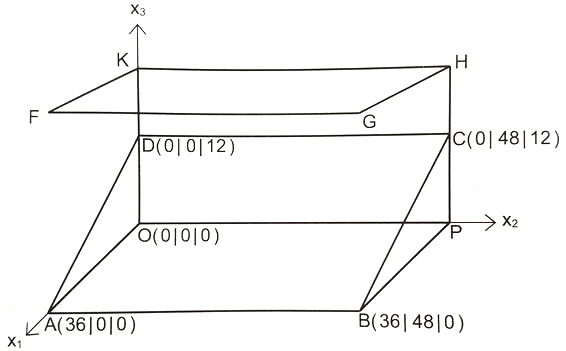
\includegraphics[width=0.5\linewidth]{tribüne.jpg}
  \end{center}
\end{figure}


\enlargethispage{2cm}

Dabei beschreibt das Rechteck ABCD mit
  $A (36|0|0)$, $ B (36|48|0)$, $C (0|48|12)$ und $ D (0|0|12) $
die Nutzfläche der Tribüne. Das Rechteck ABPO stellt die Grundfläche der Tribüne dar, das
Rechteck FGHK beschreibt die Dachfläche der Tribüne. Die Eckpunkte der Dachfläche liegen
senkrecht über den entsprechenden Eckpunkten der Grundfläche.
Die $x_1x_2 $  Ebene stellt den Erdboden dar. Die $ x_1$ – Achse zeigt nach Süden, die $x_2$ – Achse nach
Osten. Eine Längeneinheit im Koordinatensystem entspricht 1m in der Realität, d.h. die Tribüne ist
48m breit. Die Materialstärke ist bei den Rechnungen zu vernachlässigen.
\begin{enumerate}[label={\alph*)}]
\item  Bestimmen Sie eine Gleichung der Ebene N, in der das Rechteck ABCD liegt, in
Normalenform. (zur Kontrolle:$ x_1 + 3x_3 = 36 $)
    \marginpar{4 BE}
\item Berechnen Sie die Größe des Neigungswinkels der Nutzfläche gegen die Horizontale.
    \marginpar{3 BE}
\item Die Dachfläche liegt im Modell in der Ebene $E: x_1 - 6x_3 + 96 = 0.$
Ermitteln Sie die Koordinaten des Punktes G, der im Modell einen Dachflächeneckpunkt
darstellt und senkrecht über dem Punkt B liegt. (zur Kontrolle: $G (36|48|22)$)
    \marginpar{4 BE}
\item Zur Installation von Lautsprechern soll eine Metallstange so an der Tribüne befestigt
werden, dass sie an dem Punkt beginnt, der im Modell durch den Punkt $G (36|48|22)$  beschrieben wird
und an der Nutzflächenkante endet, die im Modell durch die Strecke [BC] dargestellt wird.
Aus Kostengründen soll die Stange so kurz wie möglich sein. Untersuchen Sie, ob eine 20m
lange Stange ausreicht.
    \marginpar{4 BE}
\item An der Dachflächenkante Richtung Spielstätte, im Modell dargestellt durch die Strecke
[FG], soll eine Regenrinne abgehängt werden. Ein Befestigungspunkt R liegt 2 cm
unterhalb von G. Die Lage des zweiten Befestigungspunktes wird unterhalb von F so
gewählt, dass die Regenrinne auf einer horizontalen Länge von 2 m um 2 mm abfällt. Das
Wasser soll dabei Richtung Westen abfließen. Geben Sie eine Gleichung der Geraden h an,
die den Verlauf der Regenrinne zwischen den Befestigungspunkten im Modell beschreibt.
    \marginpar{3 BE}
\end{enumerate}
\vspace{0,8cm}


\Aufgabe{(4BE + 4BE + 4BE)}

\begin{minipage}[t]{0.7\textwidth}
Die Punkte $A(7|1|1)$, $B(3|5|3)$, $C(1|1|7)$, $D$, $S_1(0|\text{--}1|0)$ und $S_2$ bestimmen als Eckpunkte eine gerade Doppelpyramide mit dem Parallelogramm $ABCD$ als gemeinsamer Grundfläche (siehe Abbildung). Beide Einzelpyramiden haben Höhen gleicher Länge.

\begin{enumerate}[label={\alph*)}]
  \item Zeige, dass das Parallelogramm $ABCD$ ein Quadrat ist.
  \item Bestimme die Koordinaten von $D$. Berechne die Koordinaten des Mittelpunktes $M$ des Quadrates $ABCD$. Ermittle die Koordinaten von $S_2$.
  \item Bestimme das Volumen der Doppelpyramide.

\end{enumerate}
\end{minipage}
\hspace*{0.75cm}
\begin{minipage}[t]{0.35\textwidth}
  \begin{figure}[H]
    \vspace{-1cm}
    \centering
    \includegraphics[width=1.2\linewidth]{Q11_2Klausur_DoppelPyramideMod.png}
  \end{figure}
\end{minipage}





\vspace{2.5cm}
\centerline{Viel Erfolg \faThumbsOUp }


\end{document}
